\documentclass[11pt,a4paper]{article}

\usepackage[a4paper,margin=2.2cm]{geometry}
\usepackage[T1]{fontenc}
\usepackage{lmodern}
\usepackage{microtype}
\usepackage{amsmath}
\usepackage{booktabs}
\usepackage{xcolor}
\usepackage{pgfplots}
\usepgfplotslibrary{groupplots}
\pgfplotsset{compat=1.18}
\usetikzlibrary{positioning,arrows.meta}
\usepackage[numbers,sort&compress]{natbib}
\usepackage{caption}
\usepackage[hidelinks]{hyperref}

\captionsetup{font=small,labelfont=bf}
\setlength{\parskip}{0.35em}

\definecolor{series}{HTML}{2A78D6}
\definecolor{inkmuted}{HTML}{52514E}
\definecolor{gridline}{HTML}{DDDCD8}
\definecolor{boxfill}{HTML}{F3F2EF}

\newcommand{\col}[1]{\texttt{#1}}
% Anything in red still has to be filled in before submitting.
\newcommand{\fillin}[1]{\textcolor{red}{#1}}
\newcommand{\groupnumber}{09}

\begin{document}

\begin{titlepage}
\centering
\vspace*{3cm}
{\large CS5344 Project Proposal\par}
\vspace{1.2cm}
{\LARGE\bfseries Steering a Tabular Diffusion Model Away from Attacks\par}
\vspace{0.5cm}
{\large Synthetic normal traffic for anomaly detection on NSL-KDD and UNSW-NB15\par}
\vspace{2cm}
{\Large Group \groupnumber\par}
\vspace{0.8cm}
\begin{tabular}{ll}
\toprule
Name & Student number \\
\midrule
Brian Kheng & A0290248B \\
Mei Xianle & \fillin{A0000000X} \\
Passion Goh Wei Ling & A0222740R \\
\bottomrule
\end{tabular}
\vfill
{\large 27 September 2026\par}
\end{titlepage}

\section{Introduction}

For each of two network intrusion datasets we get a labelled training set and have to submit a fixed number of synthetic normal rows: 40,000 for NSL-KDD and 70,000 for UNSW-NB15. These samples are used to train predefined anomaly detectors, ECOD and Isolation Forest, which are evaluated using AUPRC on hidden validation and test sets.

Since the hidden sets include attack types not present in the training data, our goal is not only to reproduce the training distribution, but to generate normal samples that provide sufficient coverage of legitimate traffic while maintaining separation from potential anomalies.

To achieve this, we propose using the mixed-type diffusion model, TabDiff~\cite{shi2025tabdiff}, on all training rows with the label as an extra column, and then sample normal rows with a guidance term that pushes each sample away from what the model associates with attacks. Section~\ref{sec:eda} looks at where the attacks actually sit in the data, Section~\ref{sec:related} covers related work, and Section~\ref{sec:approach} presents our proposed approach and evaluation strategy.

\section{Exploratory data analysis}
\label{sec:eda}

Table~\ref{tab:data} summarises the two training sets. Both are mixed-type tables with three categorical columns, and both have a little over twice as many normal rows as attacks. The numeric columns are hard to model. In NSL-KDD, 23 of the 38 numeric columns are zero in over 90\% of normal rows, and \col{src\_bytes} has a skewness of about 129 among normal rows. Eleven NSL-KDD columns and ten UNSW-NB15 columns take at most 20 distinct values (flags, TTLs and small counters), and two NSL-KDD columns, \col{num\_outbound\_cmds} and \col{is\_host\_login}, are constant. These characteristics suggest that treating all numerical features as continuous may generate unrealistic values that are not observed in the data.

\begin{table}[htb]
\centering
\small
\caption{The two training sets. Ranges and categories are taken from the normal training rows. Computed by \col{proposal/eda.py}.}
\label{tab:data}
\begin{tabular}{lrr}
\toprule
 & NSL-KDD & UNSW-NB15 \\
\midrule
Training rows (normal / attack) & 20,000 / 10,000 & 35,000 / 15,000 \\
Required synthetic rows $N$ & 40,000 & 70,000 \\
Numeric / categorical features & 38 / 3 & 39 / 3 \\
Numeric features with at most 20 distinct values & 11 & 10 \\
Constant features & 2 & 0 \\
Numeric features that are zero in over 90\% of normal rows & 23 & 4 \\
\midrule
Attacks with a category no normal row uses & 32.5\% & 1.7\% \\
Attacks with a numeric value outside the normal range & 2.0\% & 1.1\% \\
Attacks inside the normal range on every feature & 65.5\% & 97.2\% \\
Numeric features with normal-vs-attack KS distance above 0.5 & 13 & 3 \\
\bottomrule
\end{tabular}
\end{table}

Beyond these distributional challenges, we also examined whether attacks could be identified through unusual individual values or through unusual combinations of normal values. For each attack row, we checked whether any numeric value falls outside the range seen in normal rows, or whether any categorical value never appears in a normal row. In NSL-KDD, 32.5\% of attacks use a category that no normal row uses (41 of the 67 \col{service} values appear only in attacks), but only 2.0\% have an out-of-range number. The other 65.5\% sit inside the normal range on every column. This effect is more pronounced in UNSW-NB15, where 97.2\% of its attacks lie within the normal range across all columns. 

\begin{figure}[t]
\centering
\begin{tikzpicture}
\begin{groupplot}[
  group style={group size=2 by 1, horizontal sep=3.4cm},
  width=6.1cm, height=5.6cm,
  xbar, /pgf/bar width=5pt,
  xmin=0, xmax=1.08, xtick={0,0.25,0.5,0.75,1},
  xticklabel style={font=\scriptsize, color=inkmuted, /pgf/number format/fixed},
  ytick=data, yticklabel style={font=\scriptsize\ttfamily},
  y axis line style={draw=none}, x axis line style={color=gridline},
  major tick length=0pt,
  xmajorgrids, grid style={color=gridline, line width=0.4pt},
  axis x line*=bottom, axis y line*=left,
  enlarge y limits=0.07,
  nodes near coords, nodes near coords align={horizontal},
  every node near coord/.append style={font=\scriptsize, color=inkmuted, /pgf/number format/fixed, /pgf/number format/fixed zerofill, /pgf/number format/precision=2},
  title style={font=\small\bfseries, yshift=-4pt},
  xlabel style={font=\scriptsize, color=inkmuted},
  xlabel={KS distance, normal vs attack},
]
\nextgroupplot[title=NSL-KDD, yticklabels from table={figures/ks_nsl-kdd.dat}{feature}]
\addplot[fill=series, draw=none] table[x=ks, y expr=\coordindex] {figures/ks_nsl-kdd.dat};
\nextgroupplot[title=UNSW-NB15, yticklabels from table={figures/ks_unsw-nb15.dat}{feature}]
\addplot[fill=series, draw=none] table[x=ks, y expr=\coordindex] {figures/ks_unsw-nb15.dat};
\end{groupplot}
\end{tikzpicture}
\caption{The ten numeric columns of each training set whose normal and attack values differ most, measured by the two-sample Kolmogorov-Smirnov (KS) distance. Separation in UNSW-NB15 is weaker and concentrated in the TTL columns.}
\label{fig:ks}
\end{figure}

Figure~\ref{fig:ks} ranks the numeric columns by the Kolmogorov-Smirnov (KS) distance between their normal and attack values. NSL-KDD has 13 columns above 0.5, led by the byte counts while UNSW-NB15 has three, all derived from TTLs. Every UNSW-NB15 attack has \col{sttl} equal to 254 (71.5\%) or 62 (28.5\%), and both values are common in normal traffic too, at 27.1\% and 7.0\% of normal rows. These findings suggest that attacks are best detected through how often these values occur and what they co-occur with rather than through the values themselves. 

\section{Related work}
\label{sec:related}

\subsection{Unsupervised anomaly detection}

Unsupervised anomaly detection is the standard approach for network intrusion data, since labelled attack examples are scarce and attack types evolve over time. Chandola et al.~\cite{chandola2009survey} survey the classical anomaly detection methods, while Pang et al.~\cite{pang2021deep} review deep learning approaches. The two detectors used in this project, Isolation Forest~\cite{liu2008iforest} and ECOD~\cite{li2022ecod}, are both fast, unsupervised methods for tabular data. Isolation Forest identifies anomalies based on how quickly they can be isolated through random splits, while ECOD uses feature-wise tail probabilities from empirical distributions. 

However, these methods rely on different assumptions about what makes a sample anomalous. ECOD, for example, considers features independently and therefore does not explicitly model dependencies between features which is exactly the weakness Section~\ref{sec:eda} points at. ADBench~\cite{han2022adbench}, which evaluates 30 anomaly detection methods across 57 datasets, similarly finds that no unsupervised detector consistently outperforms others across datasets. The performance depends on how well a detector's assumptions match the underlying anomalies. In our setting, the detectors are already fixed, so we cannot select or tune the detector to better match the data. Instead, we can focus on controling the synthetic normal data used to train the detectors. 

\subsection{Tabular data synthesis}

This leads us to consider whether better synthetic tabular data can improve anomaly detection. Simple approaches such as SMOTE~\cite{chawla2002smote} creates new rows on the line between a row and one of its nearest neighbours. This approach is cheap, but it is limited when modelling complex relationships and categorical features. More advanced methods like CTGAN and TVAE~\cite{xu2019ctgan} model mixed-type tables with a GAN and a variational autoencoder, using mode-specific normalisation for multi-modal numeric columns and a conditional generator so that rare categories still get sampled. TabDDPM~\cite{kotelnikov2023tabddpm} brought diffusion models to tables, with Gaussian diffusion for numeric columns and multinomial diffusion for categorical ones. TabSyn~\cite{zhang2024tabsyn} instead runs score-based diffusion in the latent space of a VAE. TabDiff~\cite{shi2025tabdiff} trains a single continuous-time diffusion over both types, with masking diffusion for categorical columns and a learnable noise schedule for every column, and reports better fidelity than these earlier models on the benchmarks it tests.

Existing tabular synthesis methods are commonly evaluated based on fidelity, such as how closely synthetic data matches real-data distributions, and utility, which is how well a model trained on synthetic data performs on real data~\cite{esteban2017tstr}. Our setting differs because the downstream models are fixed to two unsupervised anomaly detectors. Therefore, reproducing the training distribution as closely as possible may not necessarily produce the synthetic data that gives the best anomaly-detection utility.

\subsection{Guidance in diffusion models}

Diffusion models also provide a way to influence the characteristics of generated samples during sampling. Classifier guidance~\cite{dhariwal2021beat} adds the gradient of a separately trained classifier to the model's score. Classifier-free guidance~\cite{ho2022cfg} drops the classifier: one network is trained with and without the condition, and sampling extrapolates from the unconditional prediction towards the conditional one, trading some diversity for samples that fit the condition more strongly. Liu et al.~\cite{liu2022composable} showed that the same arithmetic can combine several conditions, including negated ones, where subtracting the prediction for an unwanted concept moves samples away from it. Though this work was done on images and text prompts, it provides a useful direction for our problem. Rather than only learning to reproduce the observed training distribution, we can use diffusion guidance to steer generated samples away from regions associated with attacks while retaining their normal characteristics to help anomaly detectors.

\section{Intended approach}
\label{sec:approach}

Figure~\ref{fig:pipeline} shows the generator. It is one pipeline for both datasets, with only the guidance weight $w$, the training length and $N$ set per dataset.

\begin{figure}[htb]
\centering
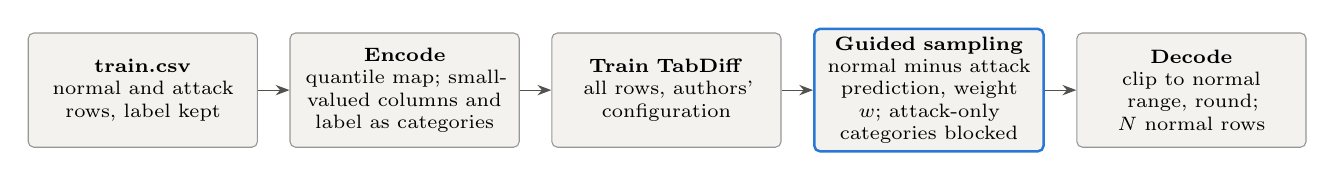
\begin{tikzpicture}[
  node distance=0.4cm,
  box/.style={draw=inkmuted!60, fill=boxfill, rounded corners=2pt, align=center, font=\scriptsize, text width=2.7cm, minimum height=1.45cm, inner sep=3pt},
  ours/.style={box, draw=series, line width=0.9pt},
  arrow/.style={-{Stealth[length=5pt]}, color=inkmuted},
]
\node[box] (data) {\textbf{train.csv}\\normal and attack rows, label kept};
\node[box, right=of data] (encode) {\textbf{Encode}\\quantile map; small-valued columns and label as categories};
\node[box, right=of encode] (train) {\textbf{Train TabDiff}\\all rows, authors' configuration};
\node[ours, right=of train] (sample) {\textbf{Guided sampling}\\normal minus attack prediction, weight $w$; attack-only categories blocked};
\node[box, right=of sample] (decode) {\textbf{Decode}\\clip to normal range, round; $N$ normal rows};
\draw[arrow] (data) -- (encode);
\draw[arrow] (encode) -- (train);
\draw[arrow] (train) -- (sample);
\draw[arrow] (sample) -- (decode);
\end{tikzpicture}
\caption{The generator. The outlined step is our addition to TabDiff.}
\label{fig:pipeline}
\end{figure}

\subsection{Backbone}

We use the TabDiff authors' model code and default configuration unchanged, and write the data handling, training loop and sampling ourselves. Before training, numeric columns with at most 20 distinct values are treated as categories, so the model can only produce values that actually occur, and constant columns are held fixed. Continuous columns are mapped to a standard normal with a quantile transform, following the TabDDPM and TabDiff preprocessing, which deals with the heavy tails from Section~\ref{sec:eda}. The label is added as one more categorical column and the model is trained on every training row, attacks included, so that it learns what attacks look like as well as normal traffic. The guidance needs both.

Training follows the authors' trainer: 8,000 epochs of AdamW with batch size 4,096, a plateau learning-rate decay, a continuous-loss weight that is annealed over training, and an exponential moving average of the weights, from which we keep the copy with the lowest training loss in the second half of training.

\subsection{Contrastive guidance}

At every sampling step we run TabDiff's denoiser $D$ twice on the current noisy row $x$, once with the label set to normal and once with it set to attack, and combine the two outputs:
\begin{equation}
\tilde{D}(x) = D(x \mid \text{normal}) + w\,\bigl(D(x \mid \text{normal}) - D(x \mid \text{attack})\bigr).
\label{eq:guidance}
\end{equation}
The same combination is applied to the logits of the categorical columns. With $w=0$ this is plain label-conditional TabDiff. With $w>0$ it is classifier-free guidance with the attack condition in place of the unconditional one, which is a negated condition in the sense of Liu et al.~\cite{liu2022composable}.

The rules ask us to explain the distribution of the generated data, and (\ref{eq:guidance}) gives a direct answer. The model's score is a linear function of the denoiser output, so (\ref{eq:guidance}) follows the score of
\begin{equation}
p_w(x) \;\propto\; p(x \mid \text{normal}) \left( \frac{p(x \mid \text{normal})}{p(x \mid \text{attack})} \right)^{w}
\label{eq:tilted}
\end{equation}
at each noise level. The samples follow the normal distribution, reweighted by how strongly each region favours normal over attack. Regions only normal traffic uses keep their mass or gain some, while regions shared with attacks, such as $\col{sttl}=254$ in UNSW-NB15, are thinned out, and $w$ sets how hard. As with classifier-free guidance, (\ref{eq:tilted}) is exact only for the noisy intermediate distributions, not for the final samples, so we also measure the final samples directly (Section~\ref{sec:eval}).

Two further constraints keep every sample a valid normal row. Categories that no normal training row uses, including the attack label itself, are blocked during sampling by setting their logits to $-\infty$, so, for example, none of the 41 attack-only NSL-KDD services ever appears in the submission. After sampling, continuous values are clipped to the range seen in normal rows and rounded to each column's precision, which keeps the output within the submission's types and ranges.

\subsection{Why this design}

Before settling on TabDiff we compared five generators with our local judge (Section~\ref{sec:eval}). Table~\ref{tab:benchmark} shows the results. On NSL-KDD no generator beats a plain bootstrap of the normal rows by more than 0.0022. TabDiff comes closest, and its samples are by far the most faithful, with a mean per-column KS distance to the normal rows of 0.014 against 0.08 to 0.14 for the other generators. TabDDPM's published sampler diverged on NSL-KDD, so its entry uses a version that clamps the predicted values while sampling.

\begin{table}[htb]
\centering
\small
\caption{Preliminary comparison of generators trained on the normal training rows with their published settings. Local combined AUPRC, averaged over two disjoint 20,000-row samples of the public datasets that exclude all coursework training rows. The first two rows are averaged over five seeds (standard deviations 0.0003 to 0.0014); the generative models ran once.}
\label{tab:benchmark}
\begin{tabular}{lrr}
\toprule
Generator & NSL-KDD & UNSW-NB15 \\
\midrule
Bootstrap of normal rows & 0.9334 & 0.5962 \\
Bootstrap plus hand-written per-column reshaping & 0.9327 & \textbf{0.6515} \\
CTGAN & 0.9351 & 0.5513 \\
TVAE & 0.9266 & 0.5918 \\
TabDDPM & 0.8910 & 0.5713 \\
TabDiff & \textbf{0.9356} & not finished \\
\bottomrule
\end{tabular}
\end{table}

On UNSW-NB15 the choice of generator matters much less than whether the labels are used. Our earlier generator, a bootstrap followed by a hand-written per-column reshaping away from attack values, gains 0.055 over the bootstrap. Applying the same reshaping to the CTGAN, TVAE and TabDDPM samples lifts them to between 0.629 and 0.643. This is what the EDA predicts: when attacks share their values with normal traffic, the synthetic data has to be shaped by where the attacks are. Contrastive guidance is a learned version of that hand-written reshaping, acting on all columns jointly instead of one at a time.

We have also checked that the guidance pushes in the right direction. With a model trained for only 300 epochs on NSL-KDD, a normal-versus-attack classifier fitted on the training data gave the samples a mean attack probability of 0.317 at $w=0$, 0.201 at $w=1$ and 0.130 at $w=2$. That confirms the direction of the push but says nothing yet about AUPRC. Full 8,000-epoch runs at $w \in \{0, 1, 2\}$ on both datasets are in progress.

\subsection{Evaluation plan}
\label{sec:eval}

We reimplemented the scoring described in the briefing as a local judge: ECOD from PyOD and scikit-learn's Isolation Forest with 500 trees for each of the seeds 0 to 9, both fitted on the submitted rows with one-hot encoded categories, and the mean of the ECOD AUPRC and the average Isolation Forest AUPRC. Some details are unspecified, such as the Isolation Forest subsample size and the categorical encoding, so we record our choices and treat the judge as a proxy. On the sample submissions it gives 0.903 for NSL-KDD, close to the public leaderboard's 0.899, but 0.664 for UNSW-NB15 against 0.383. On UNSW-NB15 we will therefore use it to compare methods, not to predict the leaderboard.

The results in Table~\ref{tab:benchmark} use rows from the public datasets. The organisers built their hidden sets from the same public data, so these rows may overlap them, and we won't use them to choose hyperparameters. To tune $w$ we will hold out a stratified 20\% of \col{train.csv}, train the generator on the other 80\%, and score on the holdout. The public data then serves only as a final check.

Guidance pushes away from the attacks the model has seen, while the hidden test set has types it hasn't. The attack type isn't released, so we will simulate unseen types by clustering the training attacks with $k$-means on the encoded features, leaving one cluster out of generator training at a time, and measuring AUPRC on the held-out cluster. If guidance helps on seen attacks but hurts on held-out clusters, we will lower $w$ or mix guided and unguided samples.

For every run we will report the two detector AUPRCs separately, per-column KS and total variation distances to the normal training rows, and the classifier attack probability above, so that score changes can be explained in terms of the data. The ablations are $w \in \{0, 0.5, 1, 2, 4\}$, sampling with and without blocked categories, and the bootstrap baseline. We will submit to Kaggle sparingly, mainly to confirm that local improvements carry over, since the public leaderboard only reflects the validation attack types.

The main risk is over-guidance. A large $w$ also removes normal traffic that happens to look like attacks, and those normal rows in the hidden set then score as anomalies, which costs precision. The holdout and held-out-cluster experiments are there to find where that starts. Training is also slow, about two hours for NSL-KDD on a laptop GPU and longer for UNSW-NB15, but the trained model is cached, so each new value of $w$ only reruns sampling, which takes minutes.

\bibliographystyle{plainnat}
\bibliography{references}

\end{document}
